\documentclass{article}
\usepackage[svgnames]{xcolor}
\usepackage[utf8]{inputenc}
\usepackage{pdfpages}
\usepackage{float}
\usepackage{fullpage} % Package to use full page
\usepackage{parskip} % Package to tweak paragraph skipping
\usepackage{tikz} % Package for drawing
\usepackage{amsmath}
\usepackage{hyperref}
\hypersetup{
    colorlinks=true,
    linkcolor=purple,
    filecolor=magenta,      
    urlcolor=pink,
}
\usepackage{amssymb}
\usepackage{bm}
\usepackage{framed}
\usepackage{amsthm}
\usepackage{listings}
\usepackage{biblatex}

\lstset{language=R,
    basicstyle=\small\ttfamily,
    stringstyle=\color{DarkGreen},
    otherkeywords={0,1,2,3,4,5,6,7,8,9},
    morekeywords={TRUE,FALSE},
    deletekeywords={data,frame,length,as,character},
    keywordstyle=\color{blue},
    commentstyle=\color{DarkGreen},
}

\addbibresource{glm-exercises.bib}

\newenvironment{lyxcode}
	{\par\begin{list}{}{
		\setlength{\rightmargin}{\leftmargin}
		\setlength{\listparindent}{0pt}% needed for AMS classes
		\raggedright
		\setlength{\itemsep}{0pt}
		\setlength{\parsep}{0pt}
		\normalfont\ttfamily}%
	 \item[]}
	{\end{list}}


\newcommand\independent{\protect\mathpalette{\protect\independenT}{\perp}}
\def\independenT#1#2{\mathrel{\rlap{$#1#2$}\mkern2mu{#1#2}}}

\newcommand{\E}{\mathrm{E}}
\newcommand{\Var}{\mathrm{Var}}
\newcommand{\Cov}{\mathrm{Cov}}
\newcommand{\Cor}{\mathrm{Cor}}

% vertical line in {bmatrix}
\makeatletter
\renewcommand*\env@matrix[1][*\c@MaxMatrixCols c]{%
 \hskip -\arraycolsep
 \let\@ifnextchar\new@ifnextchar
 \array{#1}}
\makeatother

\title{Exercises in Generalized Linear Models \\ \textbf{Week 42}}
\author{Vinnie Ko, Jonas Moss, and Ørnulf Borgan}
\date{Fall 2020}

\begin{document}
\maketitle
Exercises for the course \href{https://www.uio.no/studier/emner/matnat/math/STK3100/}{STK3100/STK4100: Introduction to Generalized Linear Models} at the University of Oslo, fall 2020. The exercises are from the textbook Alan Agresti: \textit{Foundations of Linear and Generalized Linear Models}. Wiley, 2015. ISBN: 978-1-118-73003-4. The additional exercises are available \href{https://www.uio.no/studier/emner/matnat/math/STK3100/h20/oppgaver.html}{online}. Exercises exclusively nvolving \texttt{R} are not covered.
\section*{Exercise 20}
\subsection*{(a)}
$y \in \{0,1\}$: death by SIDS\\
$x_{1} \in \{1,2,3,4,5\}$: \texttt{kohort}\\
$x_{2} \in \{1,2\}$: \texttt{kj{\o}nn}\\
$x_{3} \in \mathbb{R}^{+}$: \texttt{vekt}\\

\begin{table}[ht]
\centering
\begin{tabular}{l|l|l|l|l|l|l|}
\cline{2-7}
\multicolumn{1}{c|}{} & Additional parameters & \multicolumn{1}{c|}{Df} & \multicolumn{1}{c|}{Deviance} & \multicolumn{1}{c|}{Resid. Df} & \multicolumn{1}{c|}{Resid. Dev} & P($\vert$Chi$\vert$) \\ \hline
%
\multicolumn{1}{|l|}{NULL} & $\beta_{0}$ & & & {\color[HTML]{3531FF} $570 (=n-1)$} & {\color[HTML]{3531FF} 1101.92} & \\ \hline
\multicolumn{1}{|l|}{vekt} & $\beta_{3}$ & 1 & $259.59$ & {\color[HTML]{3531FF} $569 (=n-2)$} & {\color[HTML]{3531FF} 842.33} & $< 0.001$ \\ \hline
\multicolumn{1}{|l|}{factor(kohort)} & $\beta_{1,1}, \cdots, \beta_{1,4}$ & 4 & 314.59 & $565 (=n-6)$ & {\color[HTML]{3531FF} 527.74} & $< 0.001$ \\ \hline
\multicolumn{1}{|l|}{kjonn} & $\beta_{2}$ & 1 & 92.81 & $564 (=n-7)$ & {\color[HTML]{3531FF} 434.93} & $< 0.001$ \\ \hline
\multicolumn{1}{|l|}{vekt:factor(kohort)} & $\beta_{3:1,1}, \cdots, \beta_{3:1,4}$ & 4 & 6.37 & $560 (=n-11)$ & {\color[HTML]{3531FF} 428.56} & $0.1732$ \\ \hline
\multicolumn{1}{|l|}{vekt:kjonn} & $\beta_{3:2}$ & 1 & 0.19 & $559 (=n-12)$ & {\color[HTML]{3531FF} 428.37} & $0.6630$ \\ \hline
\multicolumn{1}{|l|}{factor(kohort):kjonn} & $\beta_{2:1,1}, \cdots, \beta_{2:1,4}$ & 4 & 15.32 & $555 (=n-16)$ & {\color[HTML]{3531FF} 413.05} & {\color[HTML]{3531FF} 0.0041} \\ \hline
\multicolumn{1}{|l|}{vekt:factor(kohort):kjonn} & $\beta_{3:2:1,1}, \cdots, \beta_{3:2:1,4}$ & 4 & 5.25 & $549 (=n-20)$ & {\color[HTML]{3531FF} 407.80} & $0.2626$\\ \hline
\end{tabular}
\end{table}

The deviance table can be used for Likelihood ratio test of model parameters. For example, if we want to test the significance of parameter $\beta_{2}$ (for the variable \texttt{kj{\o}nn}). We can read off from the deviance table:
\begin{align*}
-2\log\left(\frac{\mathrm{max}_{H_{0}}\ell\left(\beta_{0}, \beta_{1,1}, \cdots, \beta_{1,4}, \beta_{2}, \beta_{3}\right)}{\mathrm{max}_{\mathrm{full}}\ell\left(\beta_{0}, \beta_{1,1}, \cdots, \beta_{1,4}, \beta_{2}, \beta_{3}\right)}\right)
&= -2\log\left(\frac{\mathrm{max~}\ell\left(\beta_{0}, \beta_{1,1}, \cdots, \beta_{1,4}, \beta_{3}\right)}{\mathrm{max~}\ell\left(\beta_{0}, \beta_{1,1}, \cdots, \beta_{1,4}, \beta_{2}, \beta_{3}\right)}\right)\\
&= 527.74 - 424.93\\
&= 92.81\\
&> \chi_{1,0.95}^{2}\\
&= 3.84
\end{align*}


\vspace{\baselineskip}
\subsection*{(b)}
\subsubsection*{(i)}
This is similar to what we have done in  Problem 1, c) of mandatory assignment 1.\\
Interpretation of $\beta_{j}$: log of odds ratio when variable $j$ has increased by 1 unit.

\subsubsection*{(ii)}
$95\%$ confidence interval for odds ratio can be obtained by:\\
$\exp\left[\widehat{\beta}_{j}\right] \cdot \exp\left[\pm z_{0.975}\cdot SE(\widehat{\beta}_{j})\right]$

For example, for $\beta_{3}$ (\texttt{vekt}):
\begin{align*}
\exp\left[\widehat{\beta}_{3}\right] \cdot \exp\left[\pm z_{0.975}\cdot SE(\widehat{\beta}_{3})\right] = \exp\left[-0.6711\right] \cdot \exp\left[\pm 1.96\cdot 0.03758\right] = [0.4749, 0.5502]
\end{align*}


\vspace{\baselineskip}
\subsection*{(c)}
\subsubsection*{(i)}
Consider a child with covariate vector $\bm{x}_i$, and let $y_{i,j} = 1$ if the child dies of cause $j$ $(j = 1, \cdots, J)$, and $y_{i,j} = 0$ otherwise. Let $y_{i,0} = 1$ if the child survives, and $y_{i,0} = 0$ if she/he dies. Thus, $\pi_{i,j} = P(y_{i,j} = 1)$.\\

Now, we let $j=1$ correspond to SIDS. To only consider those who dies of SIDS and survive, we ignore the irrelevant part of the model and condition only on $\{y_{i,0} = 1$ \mbox{~or~} $y_{i,1} = 1\}$. This gives:
\begin{align*}
P(y_{i,1} = 1 | y_{i,0} = 1 \mbox{~or~} y_{i,1} = 1) = \frac{P(y_{i,1} = 1)}{P(y_{i,0} = 1) + P(y_{i,1} = 1)} = \frac{\pi_{i,1}}{\pi_{i,0}+\pi_{i,1}} = \frac{\exp\left[\bm{x}_{i}\bm{\beta}_{1}\right]}{1+\exp\left[\bm{x}_{i}\bm{\beta}_{1}\right]}
\end{align*}
which is a logistic regression model with the same $\bm{\beta}_{1}$ as in the multinomial logit model.\\
(See p.203 of the book.)\\

\subsubsection*{(ii)}
The advantage of using separate logistic regression for each cause, is simplicity.\\
The disadvantage is that there is no guarantee that $\sum_{j=0}^{J} \widehat{\pi}_{i,j} = 1$.


\vspace{\baselineskip}
\section*{Exercise 5.24}
\subsection*{(i)}
Since $f$ is symmetric around $0$, $F^{-1}(0.5) = 0$. Thus, if $0.5 = F(\beta_{0} + \beta_{1}x_{i})$, then $\beta_{0} + \beta_{1}x_{i} = 0$ and $x_{i} = -\frac{\beta_{0}}{\beta_{1}}$

\subsection*{(ii)}
The rate of change is $\frac{\partial \pi_{i}}{\partial x_{i}} = \frac{\partial \pi_{i}}{\partial \eta_{i}}\frac{\partial \eta_{i}}{\partial x_{i}} = f(\eta_{i})\beta_{1}$. When $\pi_{i} = 0.5$, we have $\eta_{i} = 0$ and the rate of change is $\beta_{1}f(0)$.\\

For the probit link, $f(0) = \frac{1}{\sqrt{2\pi}}$, the rate of change is $\frac{1}{\sqrt{2\pi}}\beta_{1,\mathrm{probit}}$.\\
For the logit link, $f(0) = 0.25$, the change of rate is $0.25\beta_{1,\mathrm{logit}}$.\\

Since the rate of change should be approximately the same whether the probit or logit link is used, the estimates for the logistic model should be approximately $\frac{4}{\sqrt{2\pi}} \approx 1.6$ times the estimates for the probit model.
\section*{Exercise 5.25}

\subsection*{(i)}
With complementary log-log link we have
\begin{align*}
\log\left(-\log(1-\pi_{i})\right) &= \beta_{0} + \beta_{1}x_{i}\\
\log\left(\frac{1}{1-\pi_{i}}\right) &= \exp\left[\beta_{0} + \beta_{1}x_{i}\right]\\
\frac{1}{1-\pi_{i}} &= \exp\left[\exp\left[\beta_{0} + \beta_{1}x_{i}\right]\right]\\
\pi_{i} &= 1 - \frac{1}{\exp\left[\exp\left[\beta_{0} + \beta_{1}x_{i}\right]\right]}\\
\end{align*}

When $\pi_{i} = 0.5$,
\begin{align*}
2 &= \exp\left[\exp\left[\beta_{0} + \beta_{1}x_{i}\right]\right]\\
\log\left(\log 2\right) &= \beta_{0} + \beta_{1}x_{i}\\
x_{i} &= \frac{\log\left(\log 2\right) - \beta_{0}}{\beta_{1}} = \frac{-0.3665 -\beta_{0}}{\beta_{1}}.\\
\end{align*}

The rate of change is
\begin{align*}
\frac{\partial \pi_{i}}{\partial x_{i}} &= \frac{\partial \pi_{i}}{\partial \eta_{i}}\frac{\partial \eta_{i}}{\partial x_{i}}\\
&= \frac{\exp\left[\exp\left[\beta_{0} + \beta_{1}x_{i}\right]\right] \cdot \exp\left[\beta_{0} + \beta_{1}x_{i}\right]}{\left(\exp\left[\exp\left[\beta_{0} + \beta_{1}x_{i}\right]\right]\right)^{2}}\beta_{1}\\
&= \frac{\exp\left[\beta_{0} + \beta_{1}x_{i}\right]}{\exp\left[\exp\left[\beta_{0} + \beta_{1}x_{i}\right]\right]}\beta_{1}.
\end{align*}

We find $x_{i}$ that maximizes the rate of change
\begin{align*}
\frac{\partial^{2} \pi_{i}}{\partial x_{i}^{2}} &= \frac{\partial}{\partial x_{i}}\left(\frac{\partial \pi_{i}}{\partial x_{i}}\right)\\
&= \frac{\partial}{\partial x_{i}}\left(\frac{\exp\left[\beta_{0} + \beta_{1}x_{i}\right]}{\exp\left[\exp\left[\beta_{0} + \beta_{1}x_{i}\right]\right]}\beta_{1}\right)\\
&= \frac{\beta_{1} \exp\left[\beta_{0} + \beta_{1}x_{i}\right]\exp\left[\exp\left[\beta_{0} + \beta_{1}x_{i}\right]\right] - \exp\left[\beta_{0} + \beta_{1}x_{i}\right] \exp\left[\exp\left[\beta_{0} + \beta_{1}x_{i}\right]\right] \exp\left[\beta_{0} + \beta_{1}x_{i}\right] \beta_{1}}{\left(\exp\left[\exp\left[\beta_{0} + \beta_{1}x_{i}\right]\right]\right)^{2}}\beta_{1}\\
&= \frac{\exp\left[\beta_{0} + \beta_{1}x_{i}\right] - \exp\left[\beta_{0} + \beta_{1}x_{i}\right] \exp\left[\beta_{0} + \beta_{1}x_{i}\right] }{\exp\left[\exp\left[\beta_{0} + \beta_{1}x_{i}\right]\right]}\beta_{1}^{2}\\
&= \frac{\exp\left[\beta_{0} + \beta_{1}x_{i}\right]\left(1 - \exp\left[\beta_{0} + \beta_{1}x_{i}\right]\right)}{\exp\left[\exp\left[\beta_{0} + \beta_{1}x_{i}\right]\right]}\beta_{1}^{2}\\
&= 0.
\end{align*}
So, the rate of change reaches its maximum when $\exp\left[\beta_{0} + \beta_{1}x_{i}\right] = 1$. We have then $\beta_{0} + \beta_{1}x_{i} = 0$ and $x_{i} = -\frac{\beta_{0}}{\beta_{1}}$. When $x_{i} = -\frac{\beta_{0}}{\beta_{1}}$, $\pi_{i} = 1 - \frac{1}{e} = 0.6321$.\\

\subsection*{(ii)}
Repeat i) for log-log link
\begin{align*}
-\log\left(-\log\pi_{i}\right) &= \beta_{0} + \beta_{1}x_{i}\\
\end{align*}
\section*{Exercise 5.26}
It's given that $Y_{i} \sim \mathrm{Pois}\left(\mu_{i} = \exp\left[\sum_{j}\beta_{j}x_{i,j}\right]\right)$ and $Z_{i} = I(Y_{i} > 0)$.\\
So, $Z_{i} \sim \mathrm{Bin}\left(1,\mathrm{P}(Y_{i} > 0)\right)$.\\
Notice that
$\pi_{i} = \mathrm{P}(Y_{i} > 0) = 1 - \mathrm{P}(Y_{i} \leq 0) = 1 - \mathrm{P}(Y_{i} = 0) = 1 -e^{-\mu_{i}} = 1-\exp\left[-\exp\left[\eta_{i}\right]\right] = 1-\exp\left[-\exp\left[\sum_{j}\beta_{j}x_{i,j}\right]\right]$.\\

This gives $\eta_{i} = \log\left(-\log\left(1-\pi_{i}\right)\right)$.


\input{book-exercises/exercise-6.2}
\section*{Exercise 6.3}
We use vector notation
$\bm{x}_{i} =
\begin{bmatrix}
x_{i,1}, \cdots, x_{i,p}
\end{bmatrix}$
~and~
$\bm{\beta}_{j} =
\begin{bmatrix}
\beta_{j,1}, \cdots, \beta_{j,p}
\end{bmatrix}^{\rm T}$.\\

$\pi_{i,j}$ is defined as
\begin{align*}
\pi_{i,j} =
\begin{cases}
\frac{\exp\left[\bm{x}_{i}\bm{\beta}_{j}\right]}{1+\sum_{h=1}^{c-1}\exp\left[\bm{x}_{i}\bm{\beta}_{h}\right]} ~~&\mbox{for}~~ j = 1, \cdots, c-1\\
\\
\frac{1}{1+\sum_{h=1}^{c-1}\exp\left[\bm{x}_{i}\bm{\beta}_{h}\right]} ~~&\mbox{for}~~ j = c\\
\end{cases}.
\end{align*}
Since the restriction we impose is $\bm{\beta}_{c} = \bm{0}$, I prefer to merge these two cases into one: 
\begin{align*}
\pi_{i,j} =
\frac{\exp\left[\bm{x}_{i}\bm{\beta}_{j}\right]}{\sum_{h=1}^{c}\exp\left[\bm{x}_{i}\bm{\beta}_{h}\right]} ~~&\mbox{for}~~ j = 1, \cdots, c.
\end{align*}

Thus, the rate of change is
\begin{align*}
\frac{\partial \pi_{i,j}}{\partial x_{i,k}} &= \frac{\partial}{\partial x_{i,k}}\left(\frac{\exp\left[\bm{x}_{i}\bm{\beta}_{j}\right]}{\sum_{h=1}^{c}\exp\left[\bm{x}_{i}\bm{\beta}_{h}\right]}\right)\\
&= \frac{\beta_{j,k}\exp\left[\bm{x}_{i}\bm{\beta}_{j}\right] \cdot \sum_{h=1}^{c}\exp\left[\bm{x}_{i}\bm{\beta}_{h}\right] - \exp\left[\bm{x}_{i}\bm{\beta}_{j}\right] \cdot \sum_{h=1}^{c}\beta_{h,k}\exp\left[\bm{x}_{i}\bm{\beta}_{h}\right]}{\left(\sum_{h=1}^{c}\exp\left[\bm{x}_{i}\bm{\beta}_{h}\right]\right)^2}\\
&= \frac{\exp\left[\bm{x}_{i}\bm{\beta}_{j}\right]}{\sum_{h=1}^{c}\exp\left[\bm{x}_{i}\bm{\beta}_{h}\right]}\left(\frac{\beta_{j,k}\sum_{h=1}^{c}\exp\left[\bm{x}_{i}\bm{\beta}_{h}\right] - \sum_{h=1}^{c}\beta_{h,k}\exp\left[\bm{x}_{i}\bm{\beta}_{h}\right]}{\sum_{h=1}^{c}\exp\left[\bm{x}_{i}\bm{\beta}_{h}\right]}\right)\\
&= \frac{\exp\left[\bm{x}_{i}\bm{\beta}_{j}\right]}{\sum_{h=1}^{c}\exp\left[\bm{x}_{i}\bm{\beta}_{h}\right]}\left(\beta_{j,k} -\frac{\sum_{h=1}^{c}\beta_{h,k}\exp\left[\bm{x}_{i}\bm{\beta}_{h}\right]}{\sum_{h=1}^{c}\exp\left[\bm{x}_{i}\bm{\beta}_{h}\right]}\right)\\
&= \frac{\exp\left[\bm{x}_{i}\bm{\beta}_{j}\right]}{\sum_{h=1}^{c}\exp\left[\bm{x}_{i}\bm{\beta}_{h}\right]}\left(\beta_{j,k} -\sum_{h=1}^{c}\left[\frac{\exp\left[\bm{x}_{i}\bm{\beta}_{h}\right]}{\sum_{h=1}^{c}\exp\left[\bm{x}_{i}\bm{\beta}_{h}\right]}\beta_{h,k}\right]\right)\\
&= \pi_{i,j}\left(\beta_{j,k} -\sum_{h=1}^{c}\left[\pi_{i,h}\beta_{h,k}\right]\right)\\
&= \pi_{i,j}\left(\beta_{j,k} -\sum_{h=1}^{c-1}\left[\pi_{i,h}\beta_{h,k}\right]\right)
\end{align*}

In binary case (i.e. $c = 2$), $j = 1$. So, the rate of change simplifies to 
\begin{align*}
\frac{\partial \pi_{i}}{\partial x_{i,k}} = \beta_{k}\pi_{i}(1-\pi_{i}).
\end{align*}

\section*{Exercise 6.4}
When there is 1 covariant and $c = 3$ (and assuming that the last group is the reference case),
\begin{align*}
\pi_{i,j} = \frac{\exp\left[\bm{x}_{i}\bm{\beta}_{j}\right]}{\sum_{h=1}^{c}\exp\left[\bm{x}_{i}\bm{\beta}_{h}\right]} = \frac{\exp\left[\beta_{j,0}+\beta_{j,1}x_{i}\right]}{1+\exp\left[\beta_{1,0}+\beta_{1,1}x_{i}\right]+\exp\left[\beta_{2,0}+\beta_{2,1}x_{i}\right]}.
\end{align*}
Thus,
\begin{align*}
\pi_{i,3} = \frac{1}{1+\exp\left[\beta_{1,0}+\beta_{1,1}x_{i}\right]+\exp\left[\beta_{2,0}+\beta_{2,1}x_{i}\right]}
\end{align*}
and
\begin{align*}
\frac{\partial \pi_{i,3}}{\partial x_{i}} &= \frac{\partial}{\partial x_{i}} \left(\frac{1}{1+\exp\left[\beta_{1,0}+\beta_{1,1}x_{i}\right]+\exp\left[\beta_{2,0}+\beta_{2,1}x_{i}\right]}\right)
&= -\frac{\beta_{1,1}\exp\left[\beta_{1,0}+\beta_{1,1}x_{i}\right]+\beta_{2,1}\exp\left[\beta_{2,0}+\beta_{2,1}x_{i}\right]}{\left(1+\exp\left[\beta_{1,0}+\beta_{1,1}x_{i}\right]+\exp\left[\beta_{2,0}+\beta_{2,1}x_{i}\right]\right)^{2}}.
\end{align*}

\subsection*{(a)}

If $\beta_{1,1} > 0$ and $\beta_{2,1} > 0$, then $\frac{\partial \pi_{i,3}}{\partial x_{i}} < 0$. So, $\pi_{i,3}$ is decreasing in $x_{i}$.
\subsection*{(b)}

If $\beta_{1,1} < 0$ and $\beta_{2,1} < 0$, then $\frac{\partial \pi_{i,3}}{\partial x_{i}} > 0$. So, $\pi_{i,3}$ is increasing in $x_{i}$.

\subsection*{(c)}
If $\beta_{1,1}$ and $\beta_{2,1}$ have opposite signs, $\pi_{i,3}$ can be both negative and positive. So, there is no guarantee that $\pi_{i,3}$ is monotone in $x_{i}$.
\includepdf[pages = {3,4} ]{exam-exercises/exam-2014-solution.pdf}
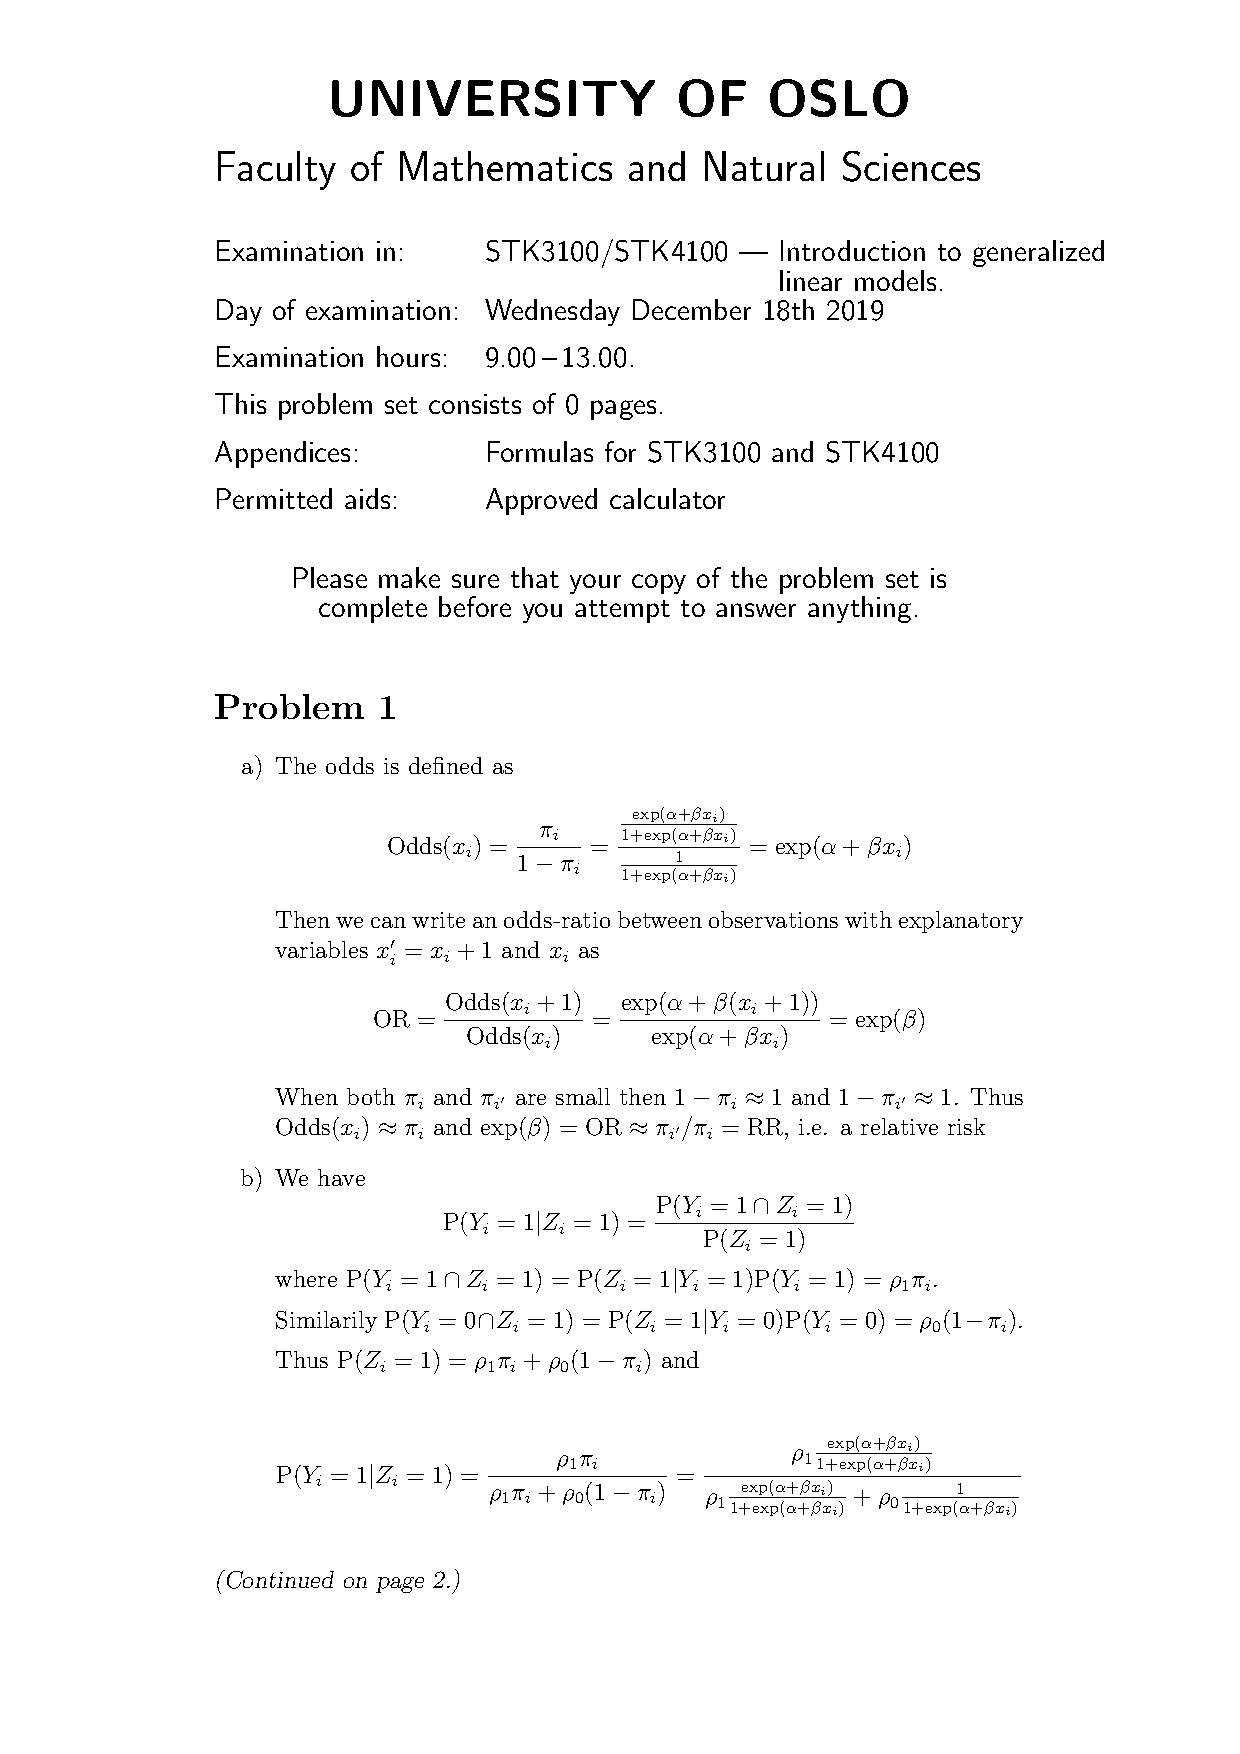
\includepdf[pages = {1,2} ]{exam-exercises/exam-2019-solution.pdf}

\printbibliography
\end{document}
